\documentclass[../DC2017114Bouma.tex]{subfiles}
\begin{document}
\graphicspath{{04_Validation/img/}}
\renewcommand{\chaptermark}[1]{\markboth{\thechapter.\ #1}{}}
\renewcommand{\sectionmark}[1]{\markright{#1}{}}
\pagestyle{fancyreport}
\cleartooddpage
\pagestyle{fancyreport}
\chapter{Numerical Validation}\label{ch:vali}
To numerically validate the theory presented in this work, some first steps are taken in creating a trajectory tracking simulation for mechanical systems with unilateral constraints and spatial friction. This chapter presents an example of such a system tracking a trajectory with simultaneous impacts. While progress is made in creating the numerical validation, the reader should be aware that it is not yet complete. More work is required to validate the LTTHS and PTTHS presented in Chapter~\ref{ch:order} and Chapter~\ref{ch:simult}, respectively, in the sense that the example discussed in this chapter does not yet contain state-and-input-dependent guards, but merely state-dependent guards.

\section{A planar 4-DOF system: RRR-robot opening a door}
In this section, an example of a mechanical system with unilateral constraints is presented, which will be simulated to validate the theory presented in this work. The system is a robot arm with three revolute joints opening a door, in a planar setting. The forward kinematics and equations of motion for that system will be presented in a concise manner. For a more thorough derivation of the equations of motion, the reader is referred to \cite{Rijnen2018b}. 

\subsection{Forward kinematics}\label{sec:5kin}
Let us now consider the system in Figure~\ref{fig:5system1}. The robot consists of four links, where link 0 is connected to the fixed world and link 3 is a foot-shaped end effector. Link 4 is a door connected to the fixed world with a torsional spring and damper. Coordinate frames are attached to each link, which are referred to as $\Psi_0$ to $\Psi_4$. The centers of mass of the links are assumed to be halfway the link, except for the center of mass of link 3. A closer look at link 3 can be seen in Figure~\ref{fig:5system2}, where the parameters $c_{3,x}$ and $c_{3,y}$ position the center of mass of link 3. Also, two additional coordinate frames $\Psi_{3a}$ and $\Psi_{3b}$ are depicted, which are attached to the contact points defined in the end effector for contact modeling. The set of contact points is given by $\mathcal{I} = \{1,2\}$, where contact point 1 and 2 are related to coordinate frames $\Psi_{3a}$ and $\Psi_{3b}$ respectively. The set of guard identifiers, which is written in binary form, is given by $\eta = \{01,10\}$, where $\gamma_{01}$ is related to contact point 1 and $\gamma^{10}$ to contact point 2. in The system is modeled without friction and trajectories with releasing motions are not considered. Therefore, the system does not contain input-dependent guard functions.

\nomenclature[G23]{$\Psi$}{A coordinate frame}%
\nomenclature[RH]{$\Hb^a_b$}{The homogeneous transformation matrix relating frame $\Psi_b$ to $\Psi_a$}%
\begin{figure}[bt!]
\centering
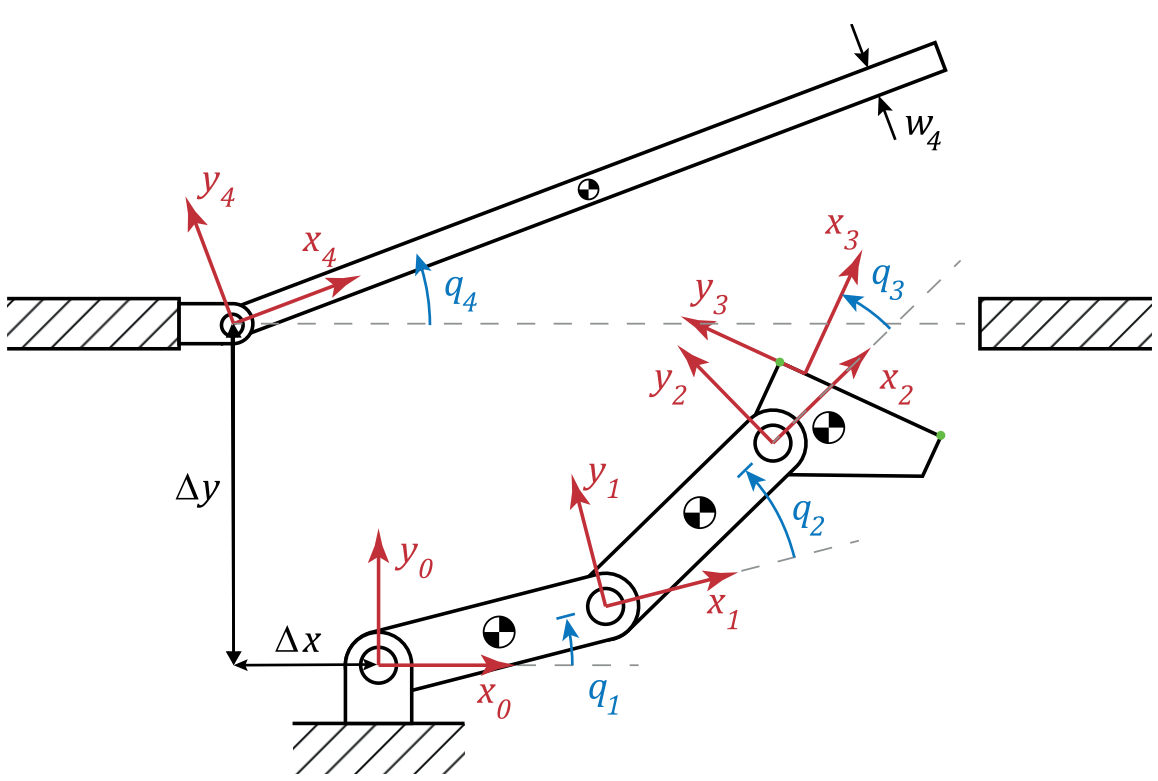
\includegraphics[width=.7\textwidth]{system.PNG}\caption{An RRR-robot and a door in top-down view. This 4-DOF planar system is used to numerically validate the theory presented in this work.}\label{fig:5system1}
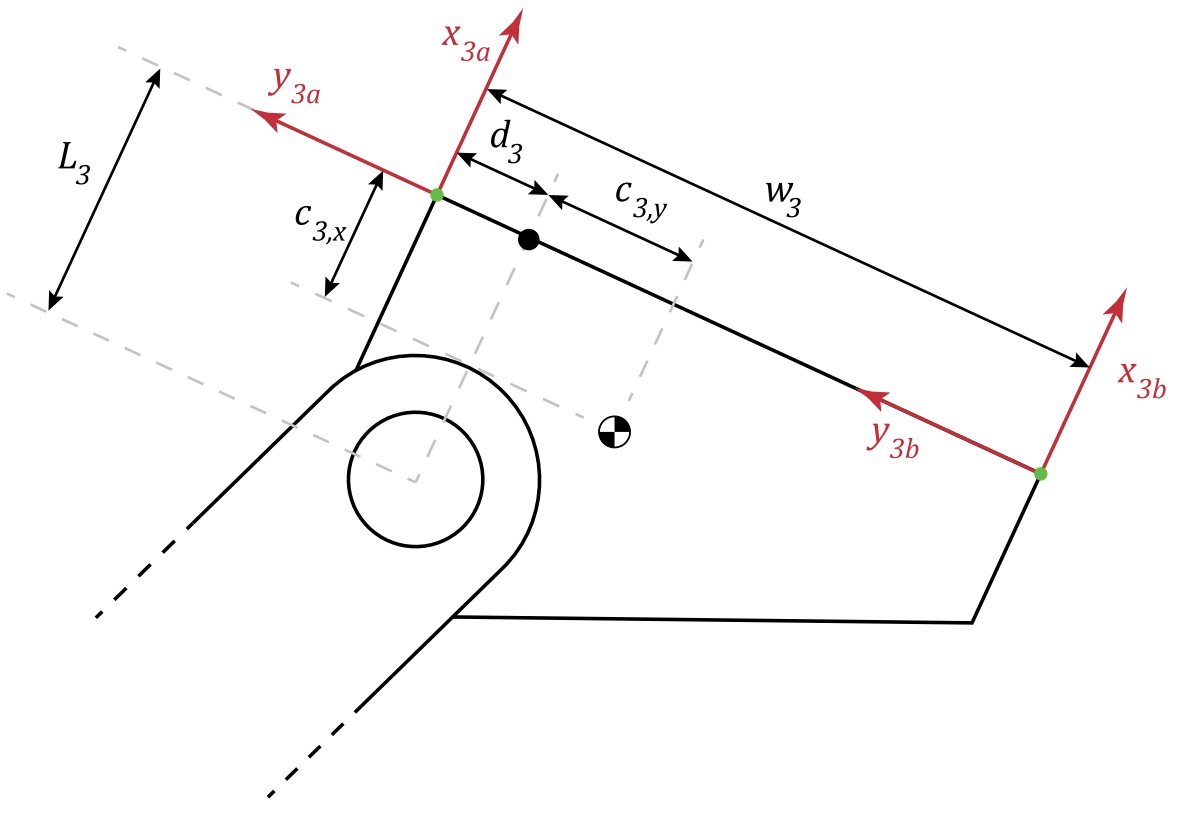
\includegraphics[width=.7\textwidth]{system2.PNG}\caption{A closer look at the foot of the RRR-robot.}
\label{fig:5system2}
\end{figure}

The generalized coordinates are defined as 
\begin{align}
\qb := \begin{bmatrix}
q_1\\q_2\\q_3\\q_4
\end{bmatrix},
\end{align}
where $\qb_i$ is the angular displacement related to the $i$-th link, as illustrated in Figure~\ref{fig:5system1}. The state of the system is then defined as
\begin{align}
\xb := \begin{bmatrix}
\qb\\\dot{\qb}
\end{bmatrix}.
\end{align}
The forward kinematics of the system are now described using homogeneous transformation matrices $\Hb^a_b$, where $\Hb^a_b$ relates coordinate frame $\Psi_b$ to coordinate frame $\Psi_a$. Since the system is in a planar setting, the transformation matrices are in the Special Euclidean group SE(2), i.e., $\Hb^a_b\in \textnormal{SE}(2)$. The transformation matrices that relate all coordinate frames to coordinate frame $\Psi_0$ are given by

\begin{align}
\Hb^0_1 &= \begin{bmatrix}
\cos(q_1) & -\sin(q_1) & L_1\cos(q_1) \\
\sin(q_1) & \cos(q_1) & L_1\sin(q_1)\\
0 & 0 & 1
\end{bmatrix},\label{eq:H01}\\
\Hb^0_2 &= \begin{bmatrix}
\cos(q_1+q_2) & -\sin(q_1+q_2) & L_1\cos(q_1) + L_2\cos(q_1+q_2) \\
-\sin(q_1+q_2) & \cos(q_1+q_2) & L_1\sin(q_1) + L_2\sin(q_1+q_2)\\
0 & 0 & 1 
\end{bmatrix},\label{eq:H02}\\
\Hb^0_3 &= \begin{bmatrix}
\cos(q_1+q_2+q_3) & -\sin(q_1+q_2+q_3) & L_1\cos(q_1) + L_2\cos(q_1+q_2) + L_3\cos(q_1+q_2+q_3) \\
-\sin(q_1+q_2+q_3) & \cos(q_1+q_2+q_3) & L_1\sin(q_1) + L_2\sin(q_1+q_2) + L_3\sin(q_1+q_2+q_3)\\
0 & 0 & 1 
\end{bmatrix},\label{eq:H03}\\
\Hb^0_4 &= \begin{bmatrix}
\cos(q_4) & -\sin(q_4) & -\Delta x \\
\sin(q_4) & \cos(q_4) & \Delta y\\
0 & 0 & 1
\end{bmatrix},\label{eq:H04}\\
\Hb^3_{3a} &= \begin{bmatrix}
1 & 0 & 0 \\
0 & 1 & d_3\\
0 & 0 & 1
\end{bmatrix},\label{eq:H33a}\\
\Hb^3_{3b} &= \begin{bmatrix}
1 & 0 & 0 \\
0 & 1 & -w_3 + d_3\\
0 & 0 & 1
\end{bmatrix}.\label{eq:H33b}
\end{align}
We now denote $x$ and $y$ the coordinates of frame $\Psi_3$ with respect to frame $\Psi_0$ in $x_0$ and $y_0$ direction respectively. We denote $\theta$ the rotation of $\Psi_3$ with respect to frame $\Psi_0$, where a positive rotation is in counterclockwise direction. The configuration of the end effector, i.e. of frame $\Psi_3$, can be obtained from \eqref{eq:H03} as
\begin{align}
\Yb:=\begin{bmatrix}
x\\y\\ \theta
\end{bmatrix} = \begin{bmatrix}
L_1\cos(q_1) + L_2\cos(q_1+q_2) + L_3\cos(q_1+q_2+q_3)\\
L_1\sin(q_1) + L_2\sin(q_1+q_2) + L_3\sin(q_1+q_2+q_3)\\
q_1+q_2+q_3
\end{bmatrix}.\label{eq:Y}
\end{align}
\nomenclature[RY]{$\Yb$}{End effector configuration}%
Since we will be considering a trajectory where the end effector makes impact with the door, the guard function associated with a open-to-closed transition, presented in Section~\ref{sec:2event}, should be evaluated. Therefore, the guard functions corresponding with contact point 1 and 2 are given by
\begin{align}
\gamma^{01} &= \hrm_{n,1}(\qb) = \begin{bmatrix} 0 & -1 & 0\end{bmatrix}\Hb^4_0\Hb^0_3\Hb^3_{3a}\begin{bmatrix}0\\0\\1\end{bmatrix}-\frac{1}{2}w_4,\\
\begin{split}
&= \Delta x\sin(q_4) + \Delta y\cos(q_4) - L_1\sin(q_1-q_4) - L_2\sin(q_1+q_2-q_4) \\
&\qquad -L_3\sin(q_1+q_2+q_3-q_4) - d_3\cos(q_1+q_2+q_3-q_4) - \frac{1}{2}w_4,
\end{split}\\
\gamma^{10} &= \hrm_{n,2}(\qb) = \begin{bmatrix} 0 & -1 & 0\end{bmatrix}\Hb^4_0\Hb^0_3\Hb^3_{3b}\begin{bmatrix}0\\0\\1\end{bmatrix}-\frac{1}{2}w_4,\\
\begin{split}
&= \Delta x\sin(q_4) + \Delta y\cos(q_4) - L_1\sin(q_1-q_4) - L_2\sin(q_1+q_2-q_4) \\
&\qquad -L_3\sin(q_1+q_2+q_3-q_4) - d_3\cos(q_1+q_2+q_3-q_4) + w_3\cos(q_1+q_2+q_3-q_4) \\ &\qquad-\frac{1}{2}w_4,
\end{split}
\end{align}
respectively. These contact distances are illustrated in Figure~\ref{fig:5guards}.
\begin{figure}[bt!]
\centering
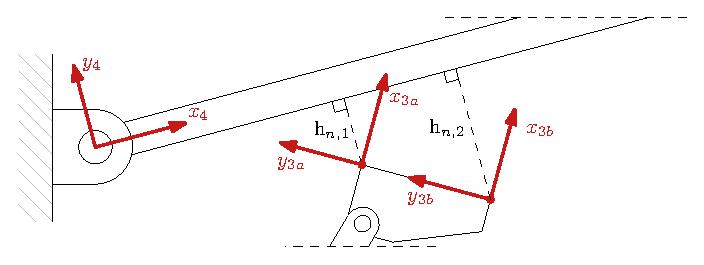
\includegraphics[width=.7\textwidth]{guards.eps}\caption{The contact distances $\hrm_{n,1}$ and $\hrm_{n,2}$ related to contact point 1 and 2.}\label{fig:5guards}
\end{figure}

\subsection{Equations of motion}
The equations of motion of the system are now presented. Since this chapter is work in progress, the system is modeled without friction. The unilateral constraints are modeled as bilateral for simplicity, and are checked for feasibility during simulation. With $\nub := \qb$ almost everywhere, the continuous dynamics of the system are given by
\begin{align}
&\Mb(\qb)\dot{\nub} + \Cb(\qb,\nub) = \Sb\ub + \sum_{\iota\in\Ic_{\text{cl}}}\wb_{n,\iota}(\qb)\lambda_{n,\iota}, &\forall \iota\in\Ic, \label{eq:5ncpcontact1}\\
&0\leq \hrm_{n,\iota}\ \bot\ \lambda_{n,\iota} \geq 0,\label{eq:5ncpcontact2}
\end{align}
with 
\begin{align}
&\hrm_{n,\iota} := \hrm_{n,\iota}(\qb),\label{eq:5h}\\
&\vrm_{n,\iota} := \wb^T_{n,\iota}(\qb) \nub.  \label{eq:5zetan}\\
\end{align}
The discrete dynamics are given by
\begin{align}
&\Mb(\qb)(\nub^+ - \nub^-) = \sum_{\iota\in\Ic_{\text{cl}}} \wb_{n,\iota}(\qb)\Lambda_{n,\iota} + \Wb_{t,\iota}(\qb)\Lambdab_{t,\iota}, \label{eq:5ncpimpact1}\\
&0\leq \vrm_{n,\iota}^+\ \bot\ \Lambda_{n,\iota} \geq 0, &\forall \iota\in\Ic_{\text{cl}},\label{eq:5ncpimpact2}
\end{align}
with 
\begin{align}
\vrm^+_{n,\iota}(\qb) &:= \wb^T_{n,\iota}(\qb) \nub^+.
\end{align}
The mass matrix $\Mb(\qb)$ is given by
\begin{align}
\Mb = \begin{bmatrix}
M_{11} & M_{12} & M_{13} & 0\\
M_{12} & M_{22} & M_{23} & 0\\
M_{13} & M_{23} & M_{33} & 0\\
0 & 0 & 0 & \overline{I}_4
\end{bmatrix},
\end{align}
with
\begin{align*}
\begin{split}
M_{11} &= \bar{I}_1 +\bar{I}_2 +\bar{I}_3 + 2L_1(L_3 - c_{3,x})m_3\cos(q_2+q_3) +2L_1 c_{3,y}m_3\sin(q_2+q_3) + L_1L_2(m_2+2m_3)\cos(q_2) \\ 
&\quad+2L_2(L_3-c_{3,x})m_3\cos(q_3) + 2L_2c_{3,y}m_3\sin(q_3),
\end{split}\\
\begin{split}
M_{12} &= \bar{I}_2 + \bar{I}_3 + L_1(L_3 - c_{3,x})m_3\cos(q_2+q_3) + L_1 c_{3,y}m_3\sin(q_2+q_3) + \frac{1}{2}L_1L_2(m_2+2m_3)\cos(q_2)\\
&\quad+ 2L_2(L_3-c_{3,x})m_3\cos(q_3) + 2L_2c_{3,y}m_3\sin(q_3)
\end{split}\\
\begin{split}
M_{13} &= \bar{I}_3 + L_1(L_3 - c_{3,x})m_3\cos(q_2+q_3) + L_1 c_{3,y}m_3\sin(q_2+q_3) + L_2(L_3-c_{3,x})m_3\cos(q_3)\\
&\quad+ L_2c_{3,y}m_3\sin(q_3),
\end{split}\\
M_{22} &= \bar{I}_2 + \bar{I}_3 + 2L_2(L_3-c_{3,x})m_3\cos(q_3) + 2L_2c_{3,y}m_3\sin(q_3),\\
M_{23} &= \bar{I}_3 + L_2(L_3-c_{3,x})m_3\cos(q_3) + L_2c_{3,y}m_3\sin(q_3),\\
M_{33} &= \bar{I}_3,\\
\bar{I}_1 &= I_1 + (\frac{1}{4}m_1 + m_2 + m_3)L_1^2,\\
\bar{I}_2 &= I_2 + (\frac{1}{4}m_2 + m_3)L_2^2,\\
\bar{I}_3 &= I_3 + m_3\left((L_3-c_{3,x})^2 + c_{3,y}^2\right),
\end{align*}
where $m_1$, $m_2$, $m_3$ are the masses of link 1 to 3, and $I_1$, $I_2$, $I_3$ are the mass moment of inertia of link 1 to 3. The spring forces, damper forces, and centripetal forces form the generalized forces vector, which is given by
\begin{align}
\Cb = \begin{bmatrix}
C_1\\C_2\\C_3\\C_4
\end{bmatrix},
\end{align}
with
\begin{align*}
\begin{split}
C_1 &=-\frac{1}{2}L_1L_2(m_2+2m_3)\left(\dot{q}_2^2 + 2\dot{q}_1\dot{q}_2\right)\sin(q_2) +L_1e(q_2+q_3)\left((\dot{q}_1 + \dot{q}_2 + \dot{q}_2)^2 - \dot{q}_1^2\right)\\ 
&\qquad+ L_2e(q_3)\left(\dot{q}_3^2 + 2\dot{q}_1\dot{q}_3 + 2\dot{q}_2\dot{q}_3\right),
\end{split}\\
C_2 &= \frac{1}{2}L_1L_2(m_2+2m_3)\sin(q_2) - L_1e(q_2+q_3)\dot{q}_1^2 + L_2e(q_3)\left(\dot{q}_3^2 + 2\dot{q}_1\dot{q}_3 + 2\dot{q}_2\dot{q}_3\right),\\
C_3 &= -L_1e(q_2+q_3)\dot{q}_1^2 - L_2e(q_3)(\dot{q}_1+\dot{q}_2)^2,\\
C_4 &= c_d\dot{q}_4 + c_k q_4,
\end{align*}
where
\begin{align*}
e(q) = m_3\left(c_{3,y}\cos(q) - (L_3-c_{3,x})\sin(q)\right).
\end{align*}
The selection matrix is $\Sb = \begin{bmatrix}\Ib_3 & \Zerob_{3 \times 1}\end{bmatrix}$. Finally, the jacobians $\wb_{n,1}^T$ and $\wb_{n,2}^T$ are defined by $\dot{\hrm}_{n,1} = \wb_{n,1}^T \dot{\qb}$ and $\dot{\hrm}_{n,2} = \wb_{n,2}^T \dot{\qb}$, which give
\begin{align}
\wb_{n,1} &= \begin{bmatrix}
a(\qb) + b(\qb) + c(\qb) + d(\qb)\\
b(\qb) + c(\qb) + d(\qb)\\
c(\qb) + d(\qb)\\
-a(\qb) - b(\qb) - c(\qb) - d(\qb) + \Delta x\cos(q_4) - \Delta y\sin(q_4)
\end{bmatrix},\\
\wb_{n,2} &= \begin{bmatrix}
a(\qb) + b(\qb) + c(\qb) + d(\qb)-w_3\sin(q_1+q_2+q_3-q_4)\\
b(\qb) + c(\qb) + d(\qb)-w_3\sin(q_1+q_2+q_3-q_4)\\
c(\qb) + d(\qb)-w_3\sin(q_1+q_2+q_3-q_4)\\
-a(\qb) - b(\qb) - c(\qb) - d(\qb) + \Delta x\cos(q_4) - \Delta y\sin(q_4)+w_3\sin(q_1+q_2+q_3-q_4)
\end{bmatrix},
\end{align}
with
\begin{align}
a(\qb) &= -L_1\cos(q_1-q_4),\\
b(\qb) &= -L_2\cos(q_1+q_2-q_4),\\
c(\qb) &= -L_3\cos(q_1+q_2+q_3-q_4),\\
d(\qb) &= d_3\sin(q_1+q_2+q_3-q_4).
\end{align}
The kinematics presented in Section~\ref{sec:5kin} and the dynamics presented in this section are first derived in \cite{Rijnen2018b}. For a more thorough derivation of the kinematics and dynamics, the reader is referred to that work. In the next section a tracking simulation for the example system is simulated and discussed. 
\section{Trajectory tracking with simultaneous impact}
\begin{itemize}
\item Hybrid toolbox
\item describe trajectory design
\item discuss attention points in trajectory design: end effector, damping constant door, accelerations around event, velocity at event
\end{itemize}
\section{Future work}


\section{Summary}

\end{document}